\section{Schwarm-Topologien}
\begin{frame}{Schwarm-Topologien}
	\begin{figure}[htbp]
		\centering
		\begin{minipage}{4cm}
			\centering
			\documentclass{standalone}

\usepackage{tikz}
\usetikzlibrary{arrows,decorations.pathmorphing,positioning,fit,petri}
\usetikzlibrary{calc,intersections,through,backgrounds,graphs}
\usetikzlibrary{patterns,decorations.pathreplacing}

\begin{document}

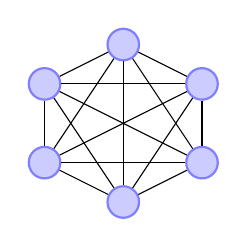
\begin{tikzpicture}
	% Styles
	[
	place/.style={circle,draw=blue!50,fill=blue!20,thick, inner sep=0pt,minimum size=4mm},
	]
                      
	% Nodes
	\node at (0,0.5)	(p1)	[place] {};
	\node at (0,1.5)	(p2)	[place] {};
	\node at (1,0)		(p3)	[place] {};
	\node at (1,2)		(p4)	[place] {};
	\node at (2,0.5)	(p5)	[place] {};
	\node at (2,1.5)	(p6)	[place] {};
	
	% Connections
	\graph[use existing nodes] {
		p1 -- p2; p1 -- p3; p1 -- p4; p1 -- p5; p1 -- p6;
		p2 -- p3; p2 -- p4; p2 -- p5; p2 -- p6;
		p3 -- p4; p3 -- p5; p3 -- p6;
		p4 -- p5; p4 -- p6;
		p5 -- p6;
	};
	

\end{tikzpicture}

\end{document}
			GBest
		\end{minipage}
		\begin{minipage}{4cm}
			\centering
			\documentclass{standalone}

\usepackage{tikz}
\usetikzlibrary{arrows,decorations.pathmorphing,positioning,fit,petri}
\usetikzlibrary{calc,intersections,through,backgrounds,graphs}
\usetikzlibrary{patterns,decorations.pathreplacing}

\begin{document}


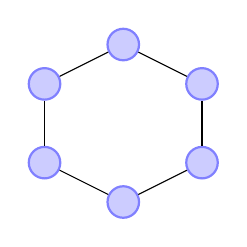
\begin{tikzpicture}
	% Styles
	[
	place/.style={circle,draw=blue!50,fill=blue!20,thick, inner sep=0pt,minimum size=4mm},
	]
                      
	% Nodes
	\node at (0,0.5)	(p1)	[place] {};
	\node at (0,1.5)	(p2)	[place] {};
	\node at (1,0)		(p3)	[place] {};
	\node at (1,2)		(p4)	[place] {};
	\node at (2,0.5)	(p5)	[place] {};
	\node at (2,1.5)	(p6)	[place] {};
	
	% Connections
	\graph[use existing nodes] {
		p1 -- p2 -- p4 -- p6 -- p5 -- p3 -- p1;
	};
	

\end{tikzpicture}

\end{document}
			LBest - Ring
		\end{minipage}
		\begin{minipage}{4cm}
			\centering
			\documentclass{standalone}

\usepackage{tikz}
\usetikzlibrary{arrows,decorations.pathmorphing,positioning,fit,petri}
\usetikzlibrary{calc,intersections,through,backgrounds,graphs}
\usetikzlibrary{patterns,decorations.pathreplacing}

\begin{document}

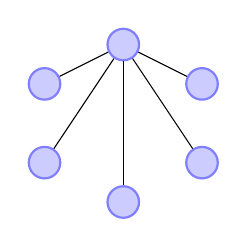
\begin{tikzpicture}
	% Styles
	[
	place/.style={circle,draw=blue!50,fill=blue!20,thick, inner sep=0pt,minimum size=4mm},
	]
                      
	% Nodes
	\node at (0,0.5)	(p1)	[place] {};
	\node at (0,1.5)	(p2)	[place] {};
	\node at (1,0)		(p3)	[place] {};
	\node at (1,2)		(p4)	[place] {};
	\node at (2,0.5)	(p5)	[place] {};
	\node at (2,1.5)	(p6)	[place] {};
	
	% Connections
	\graph[use existing nodes] {
		p4 -- p1;
		p4 -- p2;
		p4 -- p3;
		p4 -- p5;
		p4 -- p6;
	};
	

\end{tikzpicture}

\end{document}
			LBest - Wheel
		\end{minipage}
		\begin{minipage}{4cm}
			\centering
			\documentclass{standalone}

\usepackage{tikz}
\usetikzlibrary{arrows,decorations.pathmorphing,positioning,fit,petri}
\usetikzlibrary{calc,intersections,through,backgrounds,graphs}
\usetikzlibrary{patterns,decorations.pathreplacing}

\begin{document}

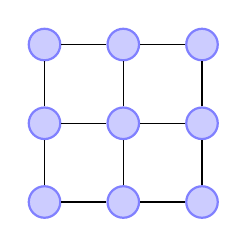
\begin{tikzpicture}
	% Styles
	[
	place/.style={circle,draw=blue!50,fill=blue!20,thick, inner sep=0pt,minimum size=4mm},
	]
                      
	% Nodes
	\node at (0,0)	(p1)	[place] {};
	\node at (0,1)	(p2)	[place] {};
	\node at (0,2)	(p3)	[place] {};
	\node at (1,0)	(p4)	[place] {};
	\node at (1,1)	(p5)	[place] {};
	\node at (1,2)	(p6)	[place] {};
	\node at (2,0)	(p7)	[place] {};
	\node at (2,1)	(p8)	[place] {};
	\node at (2,2)	(p9)	[place] {};
	
	% Connections
	\graph[use existing nodes] {
		p1 -- p2 -- p3;
		p4 -- p5 -- p6;
		p7 -- p8 -- p9;
		p1 -- p4 -- p7;
		p2 -- p5 -- p8;
		p3 -- p6 -- p9;
	};

\end{tikzpicture}

\end{document}
			LBest - Von Neumann
		\end{minipage}
	\end{figure}		
\end{frame}

\section[Zielgebiet]{Einschränkung des Zielgebiets}
\begin{frame}{Einschränkung des Zielgebiets}
	\begin{itemize}
		\item Warum eine Einschränkung ?
		\item Wie schränkt man ein Zielgebiet ein ?
		\begin{itemize}
			\item Apprallen lassen
			\item Fitness Wert auf schlechten Wert setzten
			\item Geschwindigkeit an den Grenzen auf Null setzten
		\end{itemize}
	\end{itemize}
\end{frame}

\section[Geschwindigkeit]{Maximale Geschwindigkeit}
\begin{frame}{Maximale Geschwindigkeit}
	\begin{itemize}
		\item Schnell hohe Geschwindigkeiten
		\item Lösungsansatz: Maximale Geschwindigkeit $V_{max,j}$
			\begin{equation*}
				v_{ij}(t+1) = 
				\begin{cases}
					v_{ij}(t+1) & \text{if} |v_{ij}(t+1)| < V_{max,j} \\
					V_{max,j} & \text{if} |v_{ij}(t+1)| \geq V_{max,j}
				\end{cases}
			\end{equation*} 
	\end{itemize}
\end{frame}

\section[Abbruch-kriterien]{Abbruchkriterien}
\begin{frame}{Abbruchkriterien}
	\begin{itemize}
		\item Maximale Anzahl Iterationen
			\only<1>{\\ \ \\ \ \\ 
				\colorbox{YellowGreen}{for(int i = 0, i \textless \ Maximale Anzahl Iterationen, i++)}
			}
		
		\item Schwellwert für Fitnesswert
			\only<2>{\\ \ \\ \ \\ 
				\colorbox{YellowGreen}{if(global best \textgreater \ Schwellwert) \{ ... \} }
			}
		
		\item Schwellwert für Änderung der Funktionswerte
			\only<3>{\\ \ \\ \ \\ 
				\colorbox{YellowGreen}{if(Minimale Geschwindikeit \textless \ Schwellwert)}
			}
		
		\item Schwellwert für Bewegungsbereich
			\only<4>{\\ \ \\ \ \\ \ \\
			}
		
	\end{itemize}
\end{frame}